\chapter{Grover's algorithm}

\section{What is it and why it is so important?}

[TODO: Cite: https://qiskit.org/textbook/ch-algorithms/grover.html]

Grover's search algorithm is a quantum algorithm framework, that takes a user-defined solution verifier algorithm (the oracle) and turns it into a $\Theta(\sqrt{N})$ solver. This provides a quadratic speedup over the classical brute force equivalent.

Many sources call this a database search algorithm, since in Grover's original paper it was described as such. However, the 'database' here is an abstract entity, that represents the entire domain of the problem, while the so-called 'marked' elements are the correct solutions in this domain, for which the oracle would return a 'YES' answer. Using the terms 'problem domain' instead of 'database', 'verifier algorithm' insead of 'oracle' and 'solutions' instead of 'marked elements' makes Grover's importance and connection to the P versus NP problem clearer and the details of the algorithm easier to understand.

Another common description of Grover's search algorithm is that it can solve 'unstructured search problems'. What they mean by this is that the algorithm doesn't construct a solution by iterating over partial solutions or improving a non-solution step-by-step. Constrast this with for example how Prim's minimum spanning tree algorithm iterates on partial solutions by connecting the remaining vertices of the graph one at a time. This requires knowledge of the graph and knowledge of how to build a minimal spanning tree one vertex at a time.

Grover doesn't need to know the structure of the original problem, the relationship between partial solutions or how to improve non-solutions. It only needs to know how to verify a solution. It starts by taking all of the entities from the problem's domain with uniform distribution.

\begin{figure}[H]
    \centering
    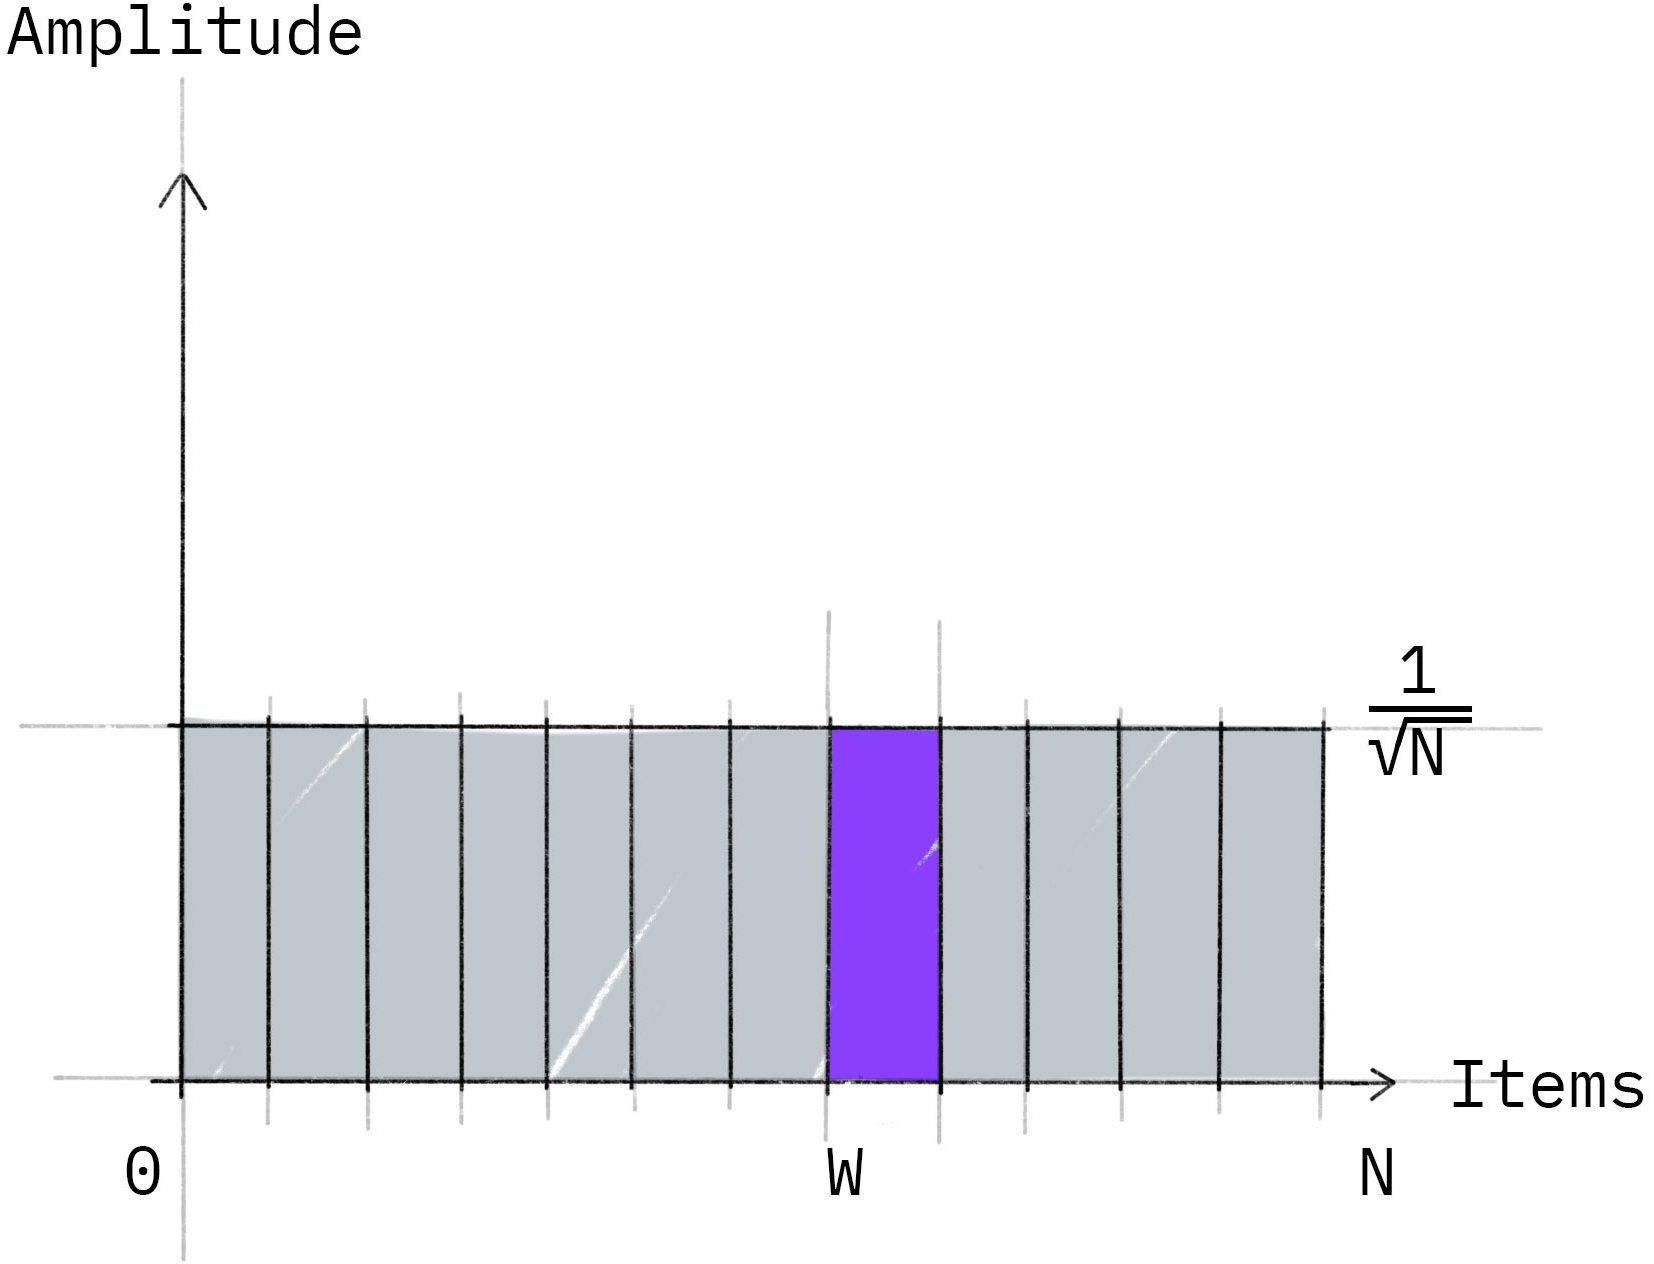
\includegraphics[width=0.5\linewidth]{content/assets/03_grovers_algorithm/grover_uniform.jpg}
    \caption{Grover starts out with the uniform distribution}
    \label{fig:grover_uniform}
\end{figure}

Then, it uses the verifier algorithm in a process to manipulate their probabilities until the correct entities' probabilities are very high, while the incorrect entities' probabilities are very low. This process is called amplitude amplification.

\begin{figure}[H]
    \centering
    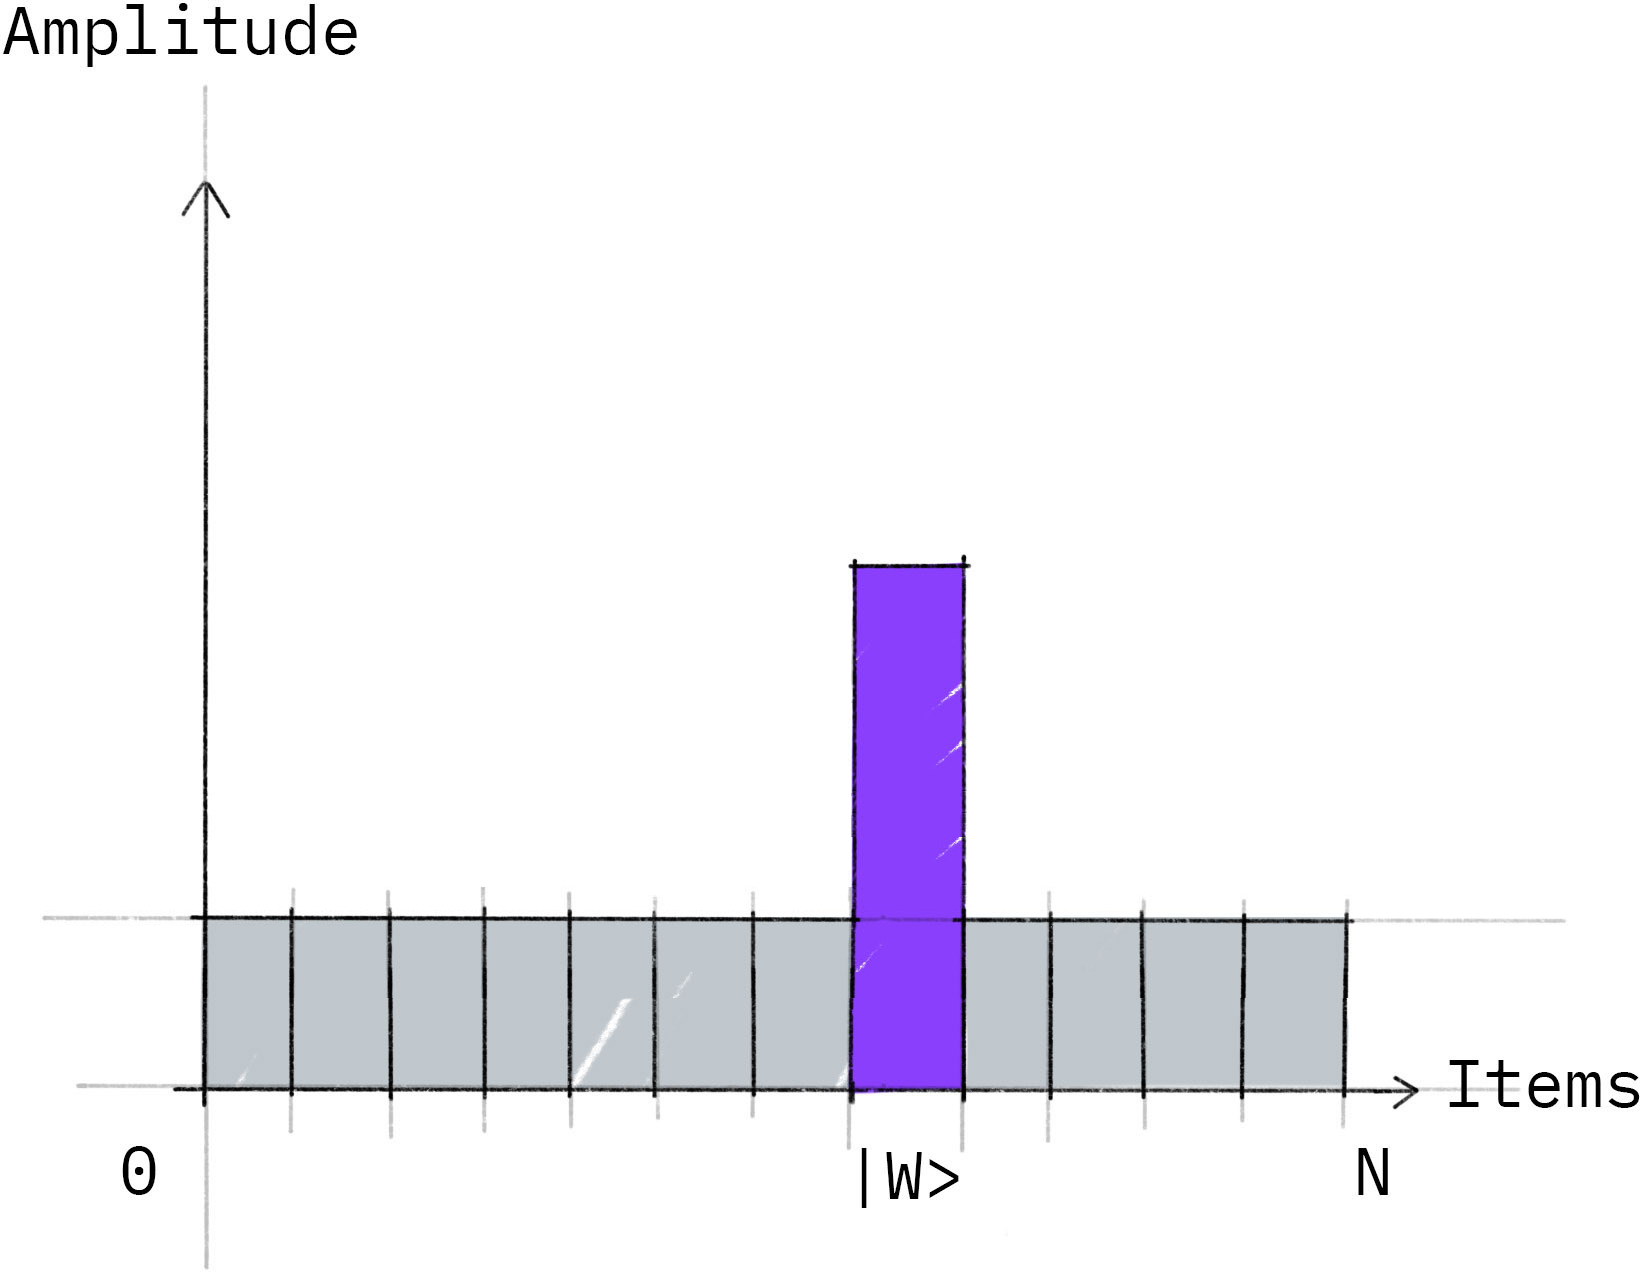
\includegraphics[width=0.5\linewidth]{content/assets/03_grovers_algorithm/grover_final.jpg}
    \caption{Grover amplifies the amplitude(s) of the correct solution(s)}
    \label{fig:grover_uniform}
\end{figure}

Finally, it samples from this probability distribution, which results in a correct solution entity with a high chance.

Working with a probability distribution over an exponentially large set of entities is only possible in a memory-efficient way on a quantum computer, thanks to the quantum physical nature of qubits.

A register of classical bits can only represent a single entity (encoded as a binary number), we would need separate registers to represent a set and we can only operate on the entire set in a linear fashion, one register at a time. In contrast, a register of quantum bits, or 'qubits' itself can represent a set of entities (a set of binary numbers) from the domain using the quantum physical phenomenon of superposition with a probability distribution over these elements.

The manipulation of these probabilities happens using quantum operators or gates, which are the basis of all quantum algorithms on gated general-purpose quantum computers.

However, we do not have access to this probability distribution or the high probability elements in it. The only thing we can do is read the register, which is an operation that samples a single entity from the current probability distribution in the register, destroying it in the process. We are unable to 'iterate' the contents of the register or know what the probability of the resulting element was from the sampling.

This is the reason why quantum parallelism is not as trivial as the name suggests: while we can run the computation itself in parallel, gaining access to the information that we stored in the register is difficult and destructive. Amplitude amplification is a technique that we use to fix this problem, however it requires $O(\sqrt{N})$ time, where $N$ is the size of the problem's domain, where $N=2^n$ if the quantum register has $n$ qubits.

One of the most important property of quantum registers is that they can even represent probability distributions, even ones where the individual qubits are \textbf{not independent}. This is called quantum entanglement.

The simplest forms of quantum entanglement are Bell states, which can occur between two qubits. In one of these Bell states, the probability distribution of our 2 qubit quantum registers is "$00$" with $50\%$ probability and "$11$" with $50\%$. Reading the contents of just the first qubit will result in a $50\%$ chance of reading a $0$ and a $50\%$ chance of reading a $1$. However, once we know the result from the first qubit, we can be $100\%$ sure, that when we sample the second qubit, we will get the same number as a result from it.

\section{The Task: Generalization of the Sudoku puzzle}

In the original Sudoku puzzle, we have a $(3^2\cdot{}3^2)$ table, that must be filled with numbers between $1$ and $9$. A correct solution to a puzzle is where each row, column and distinct $(3\cdot{}3)$ square has unique numbers.

\begin{figure}[H]
    \centering
    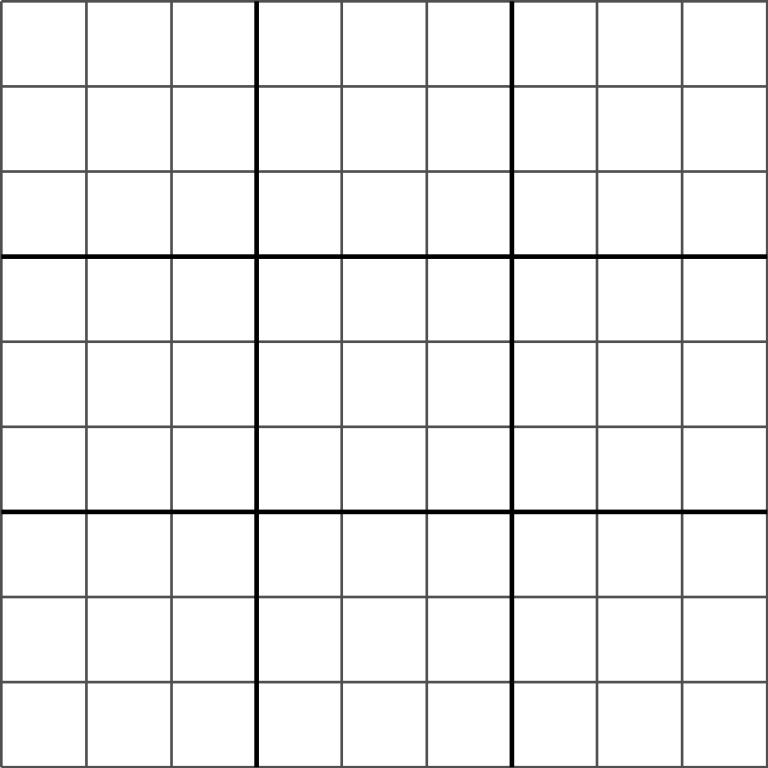
\includegraphics[width=0.7\linewidth]{content/assets/03_grovers_algorithm/sudoku_3.png}
    \caption{Empty Sudoku puzzle (Source:  \href{https://en.wikipedia.org/wiki/File:Sudoku_Puzzle_by_L2G-20050714_standardized_layout.svg}{Wikimedia Commons})}
    \label{fig:my_label}
\end{figure}

\begin{figure}[H]
    \centering
    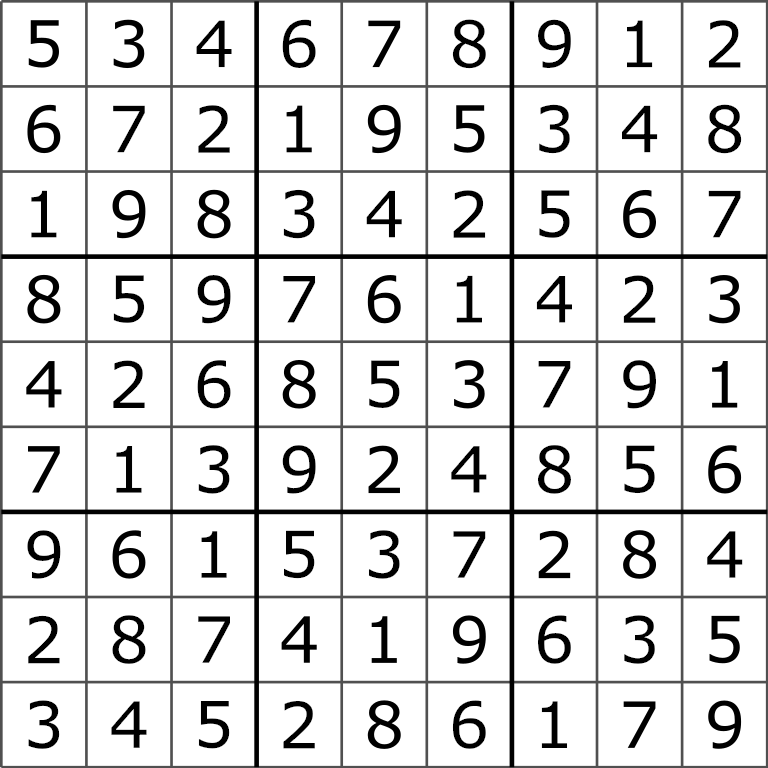
\includegraphics[width=0.7\linewidth]{content/assets/03_grovers_algorithm/sudoku_3_solved.png}
    \caption{One possible Sudoku solution (Source:  \href{https://en.wikipedia.org/wiki/File:Sudoku_Puzzle_by_L2G-20050714_solution_standardized_layout.svg}{Wikimedia Commons})}
    \label{fig:my_label}
\end{figure}

In order demonstrate memory usage scaling, I generalize this Sudoku to a table of size $(n^2\cdot{} n^2)$, where each row, column and $(n\cdot{}n)$ distinct subsquare of the table must be a unique number from the $[1, n^2]$ interval.

The only solution for $n=1$ is trivial.

\begin{figure}[H]
    \centering
    
\includegraphics[width=0.077\linewidth]{content/assets/03_grovers_algorithm/sudoku_1.png}
    \caption{Empty Sudoku puzzle $n=1$}
    \label{fig:my_label}
\end{figure}

\begin{figure}[H]
    \centering
    
\includegraphics[width=0.077\linewidth]{content/assets/03_grovers_algorithm/sudoku_1_solved.png}
    \caption{Solved Sudoku puzzle $n=1$}
    \label{fig:my_label}
\end{figure}

An example solution for $n=2$.

\begin{figure}[H]
  \centering
  \begin{subfigure}{.5\linewidth}
    \centering
    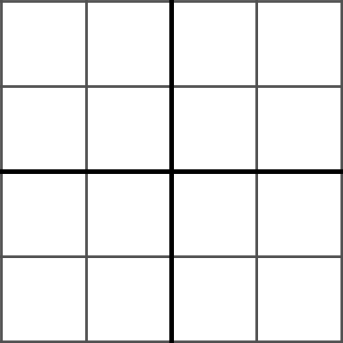
\includegraphics[width=0.622\linewidth]{content/assets/03_grovers_algorithm/sudoku_2.png}
    \caption{Empty Sudoku puzzle $(n=2)$}
  \end{subfigure}
  \begin{subfigure}{.5\linewidth}
    \centering
    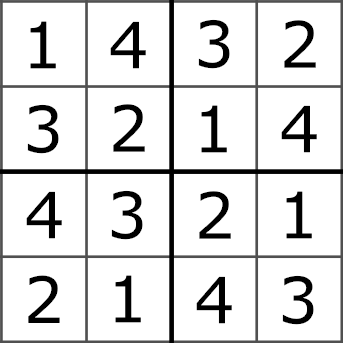
\includegraphics[width=0.622\linewidth]{content/assets/03_grovers_algorithm/sudoku_2_solved.png}
    \caption{Solved Sudoku puzule}
  \end{subfigure}
  \caption{}
\end{figure}




$n=3$ is normal Sudoku.

And an example for $n=4$ is the following:




[TODO]



\section{Designing a quantum algorithm solver based on Grover's search}

The first step is to encode the problem using quantum registers.

